% !TeX engine = xelatex
% !TeX spellcheck = en-US
% adjust to 16:9 for displays. you can just use \documentclass[handout]{ctexbeamer} for notes
\documentclass[aspectratio=169]{ctexbeamer}
\usepackage{ctex}
\usepackage{booktabs}
\usepackage{svg}
\usepackage{pdfpages}
\usepackage{fontspec}
\usepackage{fontawesome}
\usepackage[style=authortitle-comp,backend=bibtex]{biblatex}
\usecolortheme{seagull}
\setbeamertemplate{sidebar right}{}
\setbeamertemplate{footline}{%
	\hfill\usebeamertemplate***{navigation symbols}
	\hspace{1cm}\insertframenumber{}/\inserttotalframenumber}
\title{针对时间序列分类(TSC)的深度模型}
\subtitle{Deep Learning for Time Series Classification \footfullcite{fawaz2019deep}}
\author{Xinyi Li}
\date{\today}

\addbibresource{ref.bib}

\begin{document}
\begin{frame}
	\titlepage
\end{frame}

\begin{frame}{Overview}
  \tableofcontents
\end{frame}

\section{问题背景描述}

\begin{frame}{Problem Description}
	\framesubtitle{univariance/multi-variance/panel}
	\begin{center}
		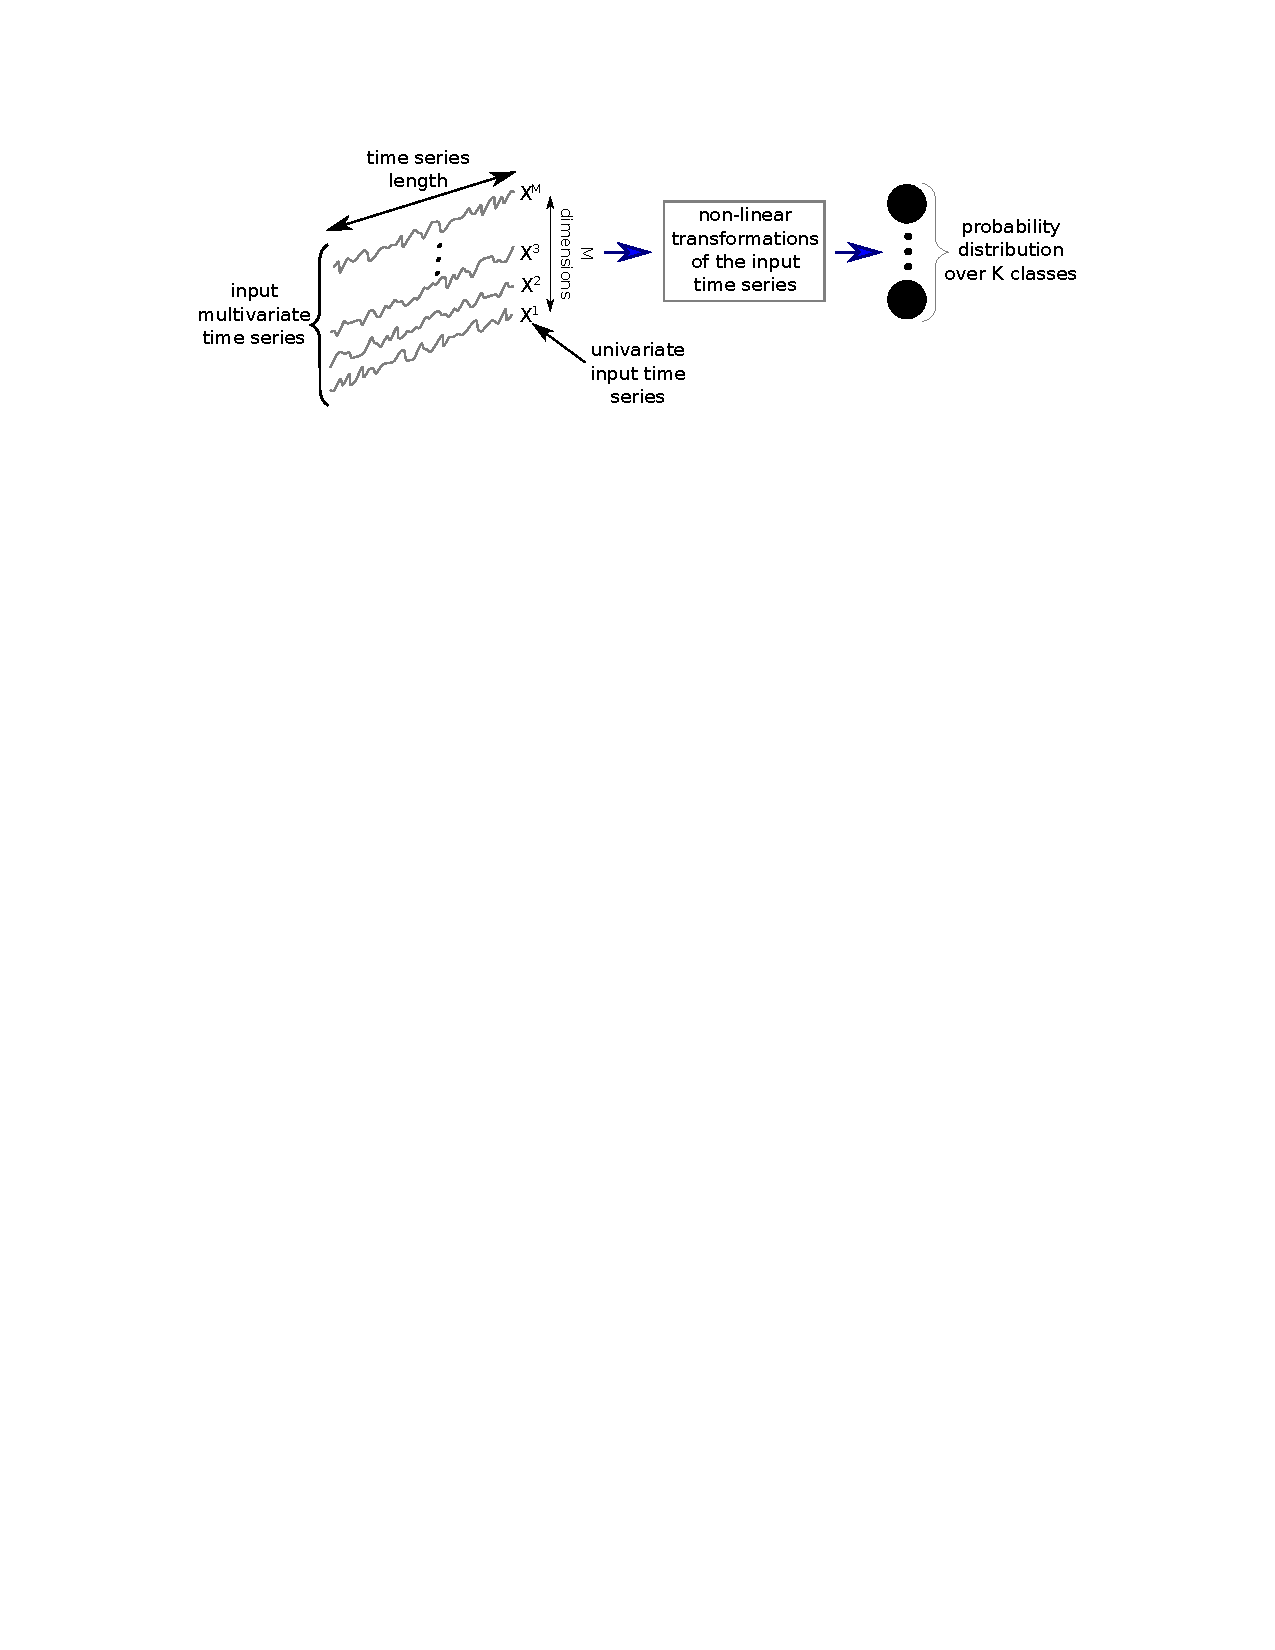
\includegraphics[width=\textwidth]{figure/base_formula}
	\end{center}
\end{frame}

\begin{frame}{Different Univariate Learning Tasks}
	\begin{columns}

		\column{.47\textwidth}
		\begin{block}{MTS}
			\begin{itemize}
				\item different measurements of the \textbf{same} instance
				\item \textbf{high correlation}
				\item feeding features
			\end{itemize}
		\end{block}

		\column{.47\textwidth}
		\begin{block}{panel data}
			\begin{itemize}
				\item the same measurements on \textbf{different} instances
				\item i.i.d. assumption
				\item feeding sku/store/...
			\end{itemize}
		\end{block}
	\end{columns}
\end{frame}



\section{Strong Baseline}
\begin{frame}{HIVE-COTE\footfullcite{lines2016hive}:}
	\framesubtitle{\textbf{SOTA} classic algorithm \footfullcite{bagnall2017great}: Collective of Transformation based \textbf{Ensembles} (COTE) with a Hierarchical Vote system}
	\begin{enumerate}
		\item Elastic Ensemble(\textbf{EE}): combination of 1-NN classifiers using different measurements
		\item Shapelet Transform Ensemble(\textbf{ST}): top $k$ shaplets (independent phase short pattern)
		\item Bag-of-SFA-Symbols (\textbf{BOSS}) Ensemble: shapelets based on presence or absence
		\item Time Series Forest (\textbf{TSF}): trained on selected $3 \sqrt{m}$ features
		\item Random Interval Features (\textbf{RIF}): spectral component of \textit{Flat-COTE}
	\end{enumerate}
\end{frame}

\begin{frame}{HIVE-COTE Algorithm\footnote{\url{https://github.com/TonyBagnall/py-hive-cote}}}
	\framesubtitle{ensemble of ensembles: ref to Flat-COTE}
	\begin{center}
		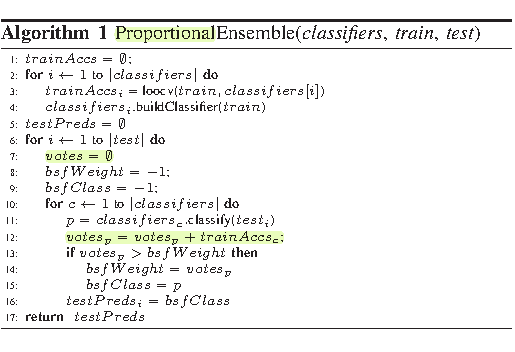
\includegraphics[width=.7\textwidth]{figure/flat_cote_algo}
	\end{center}

\end{frame}


\section{深度模型结构}

\subsection{MLP/DNN}
\begin{frame}{MLP/DNN}
	\framesubtitle{Multi Layer Perceptrons/Fully-Connected(FC) Network}
	The Simplest DNN (e.g. \texttt{keras.Layers.Dense})
	$$\mathbf{X}_{i+1} = \sigma (\mathbf{W}_i \mathbf{X}_i + b_i)$$
	Final ($l$-th) layer activate function: softmax
	$$\hat {y} _{k} (\mathbf{X}_{l-1}) = (e^{\mathbf{W}_k \mathbf{X}_{l-1} + b_k}) /
	(\sum_{i=1}^{K} {e^{\mathbf{W}_i \mathbf{X}_{l-1} + b_i}})$$
	Objective loss:  categorical cross entropy
	$$Loss(\textbf{X}) = - \sum_{i=1}^{K}{y_i} \log {\hat y}_i$$
	minimized to learn the weights using \textbf{gradient descent} method
\end{frame}

\subsection{FCN}
\begin{frame}{FCN\footfullcite{gamboa2017deep}}
	\framesubtitle{Fully Convolutional Neural Network}
	\begin{center}
		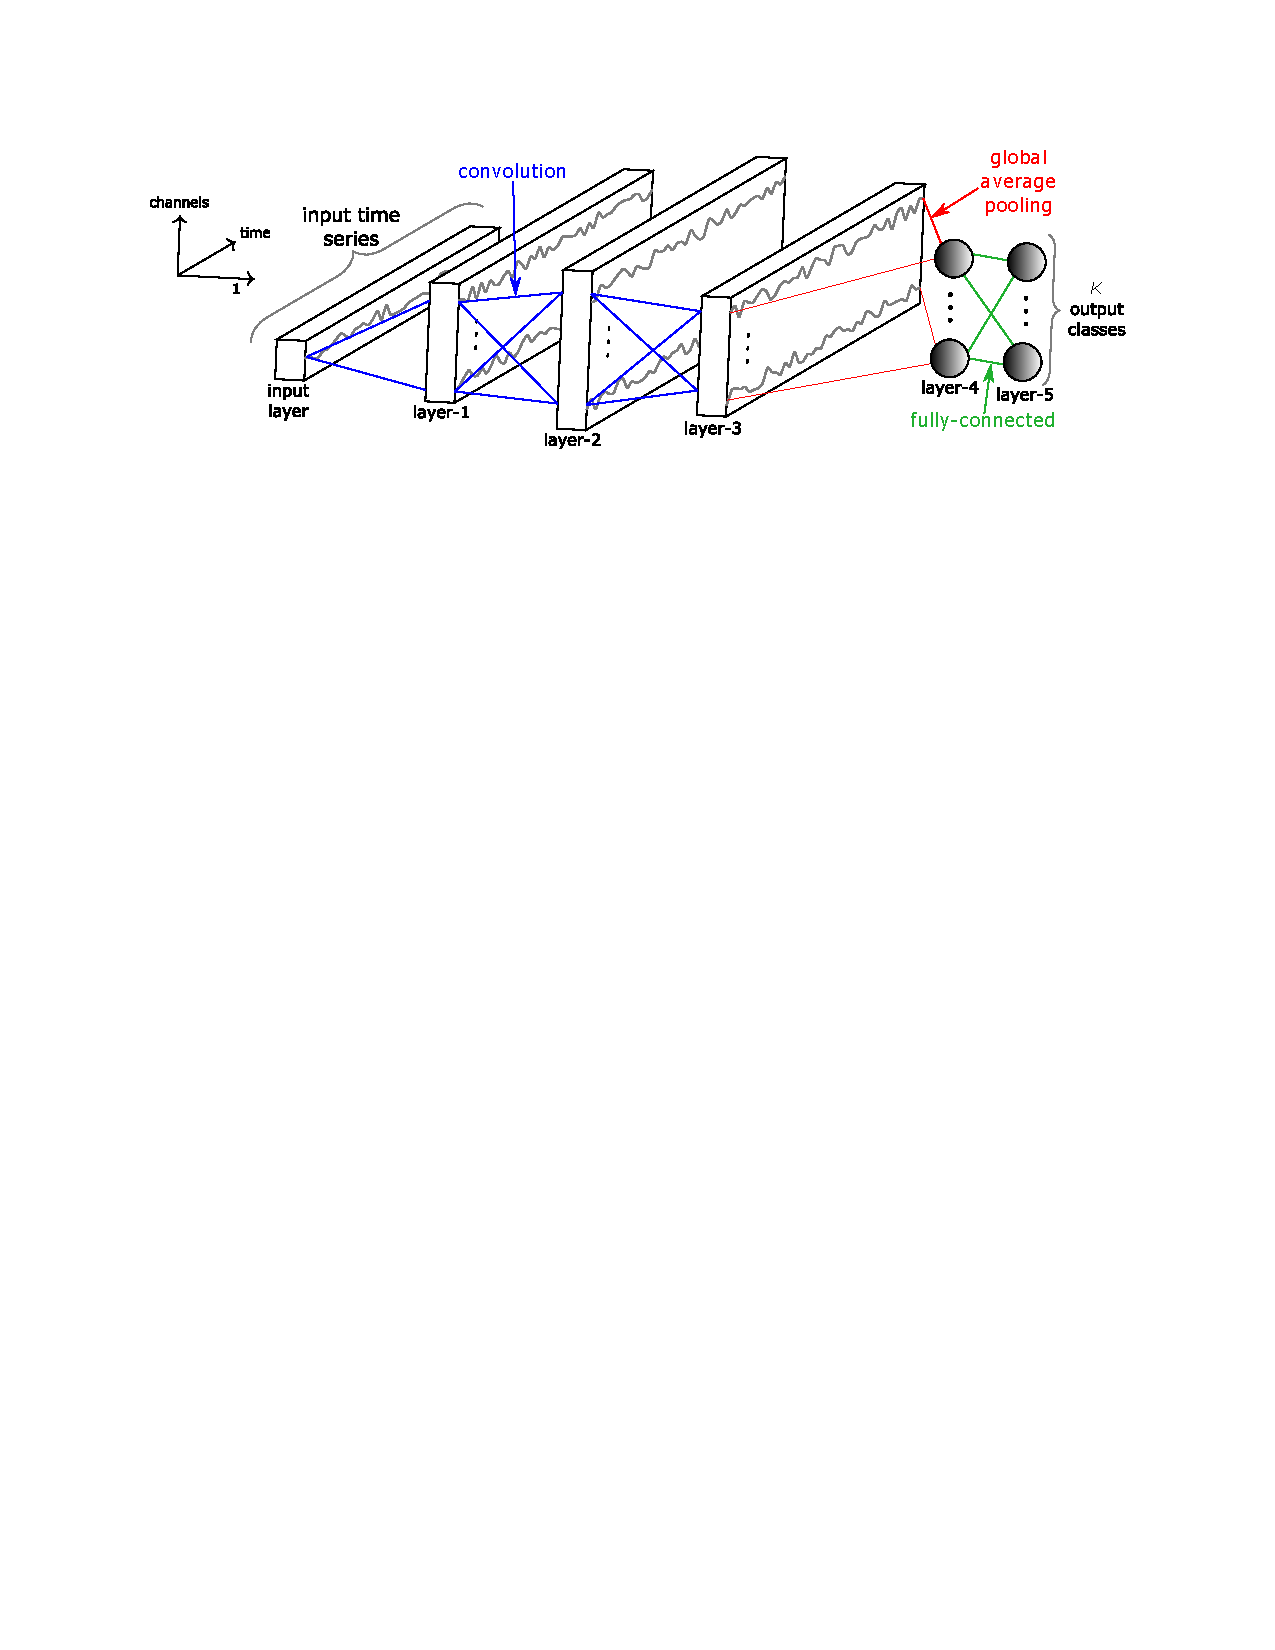
\includegraphics[width=\textwidth]{figure/fcnn}
	\end{center}
	convolution layer ($\forall$ time stamp $t$ shares filter $\color{blue}{\omega}$ with length $l$)
	$$\mathbf{C}_t = \sigma ({\color{blue}{\omega}}* \mathbf{X}_{t-l/2:t+l/2} + {\color{blue}{b}}) | \forall t \in [1,T ]$$
\end{frame}

\subsection{ResNet}
\begin{frame}{ResNet\footfullcite{wang2017time}}
 \framesubtitle{Residual Network}
 \begin{center}
 	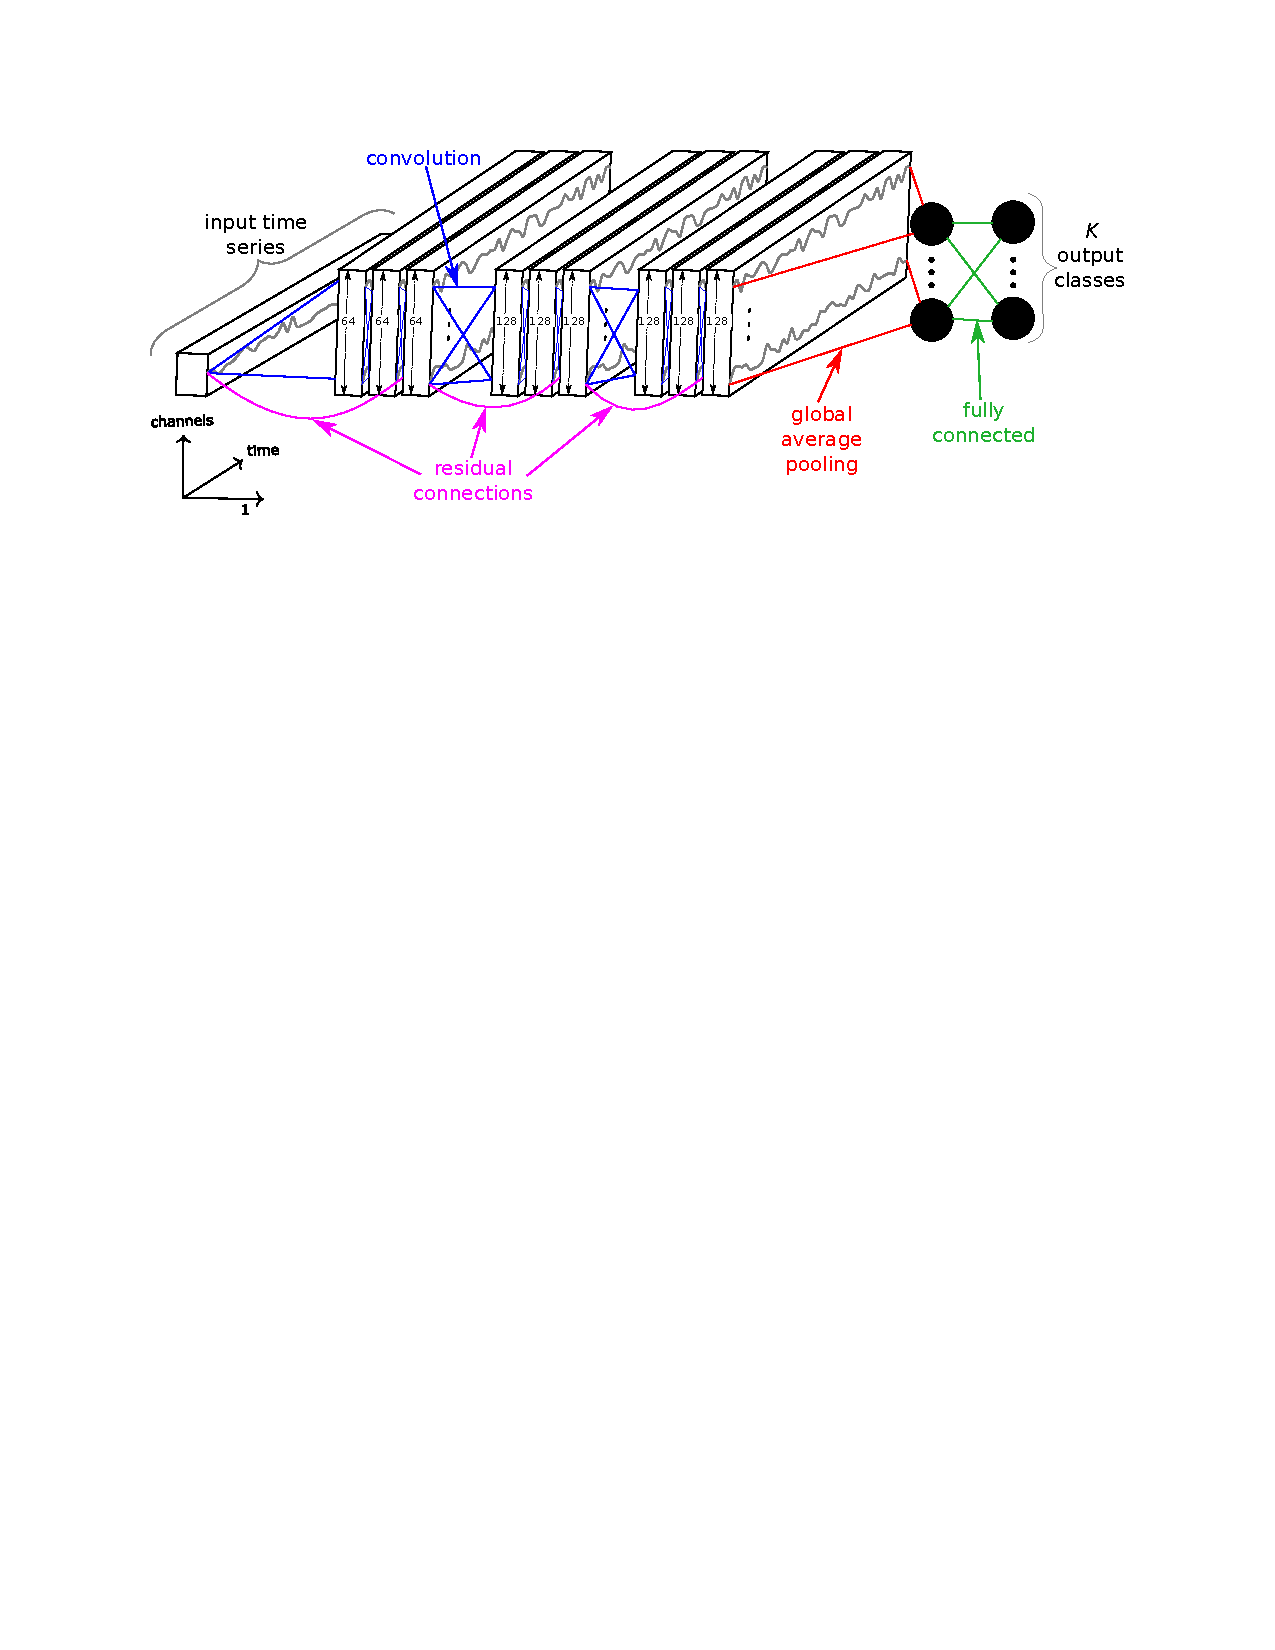
\includegraphics[width=.8\textwidth]{figure/resnet}
 \end{center}
\end{frame}

\subsection{Encoder}

\begin{frame}{Encoder\footfullcite{serra2018towards}}
	\framesubtitle{Hybrid deep CNN based on FCN}
	Modified from FCN
	\begin{itemize}
		\item GAP layer $\to$ attention layer ({\color{red}{careful design for pre-train}})
		\item normalization for each Conv layer output:
		\begin{enumerate}
			\item ReLU $\to$ PReLU activation function (+ parameter)
			\item + dropout regularization
			\item + max pooling
		\end{enumerate}
		\begin{center}
			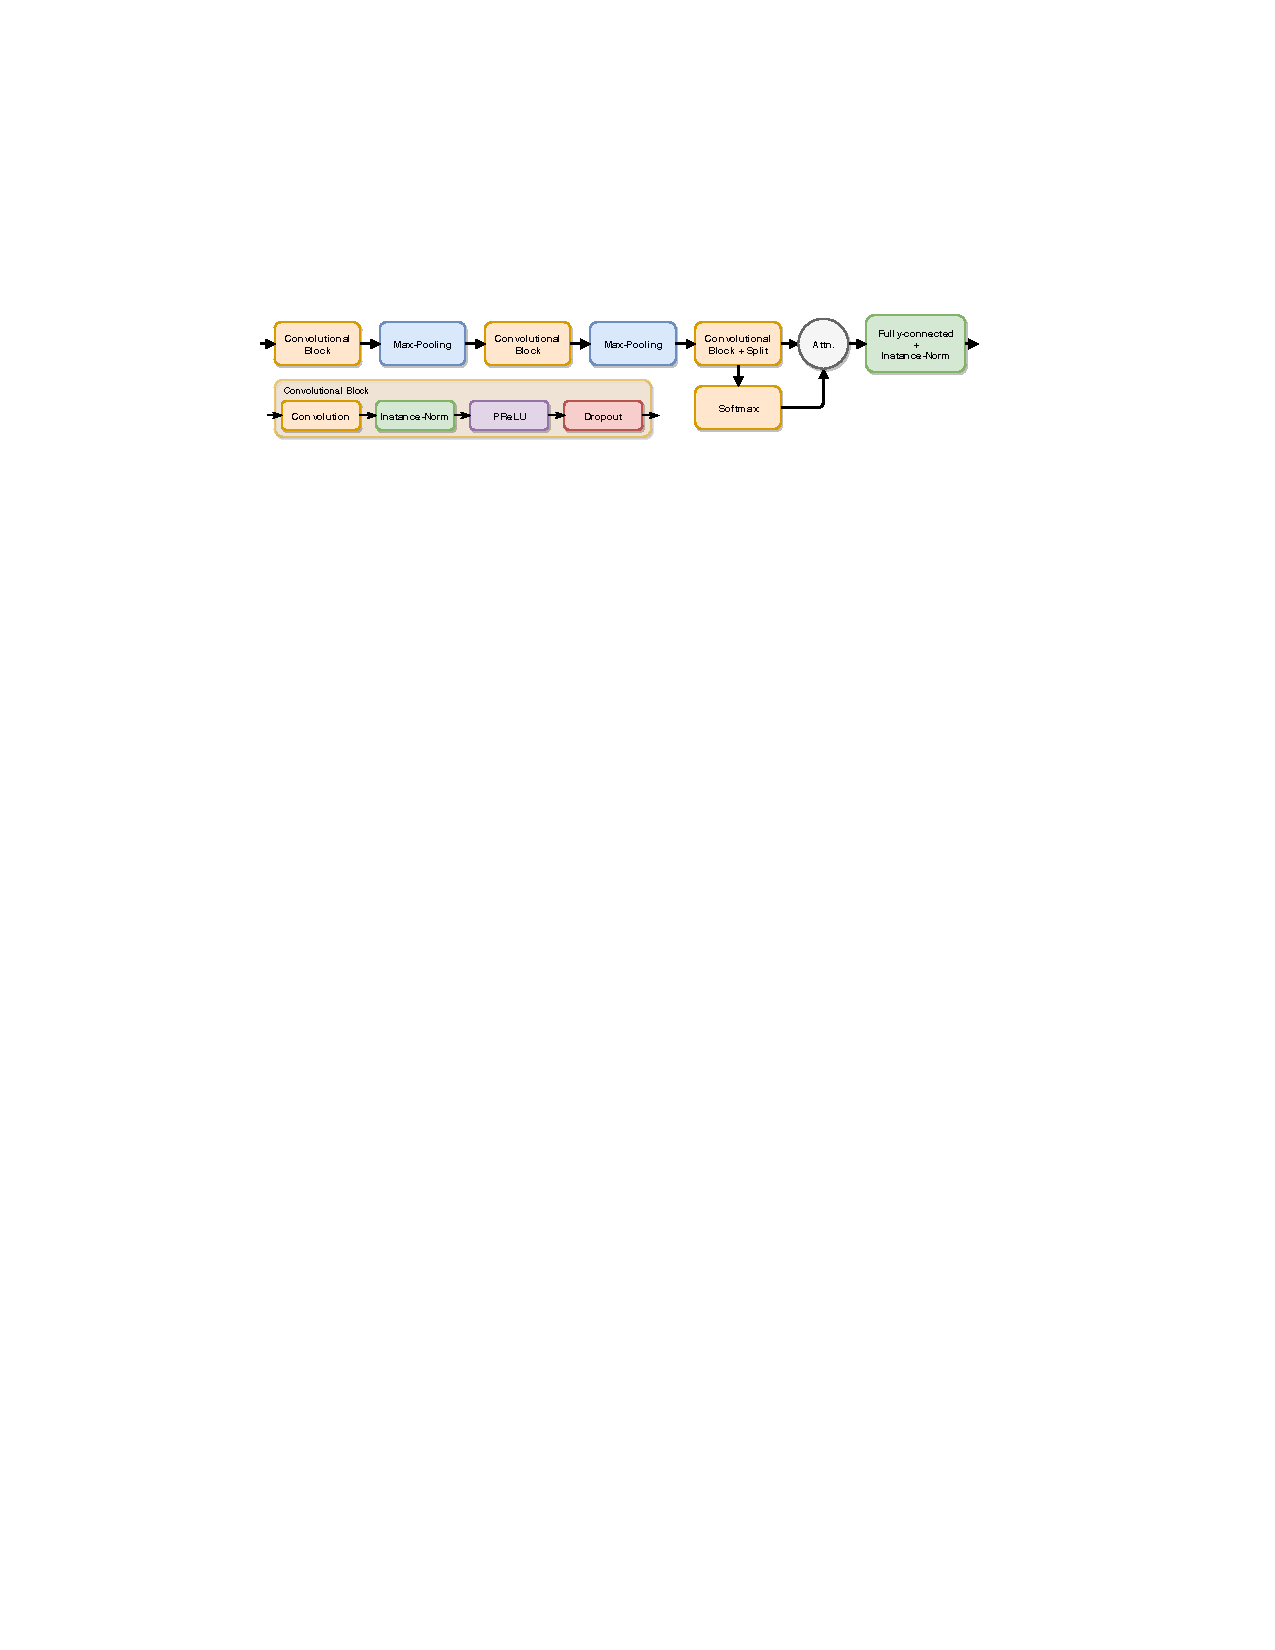
\includegraphics[width = .95\textwidth]{figure/encoder}
		\end{center}
	\end{itemize}
\end{frame}

\subsection{MCNN}
\begin{frame}{MCNN\footfullcite{cui2016multi}}
	\framesubtitle{Multi-scale Convolutional Neural Network}
	\begin{columns}
		\column{.45\textwidth}
		\begin{block}{Similar to Traditional CNN:}
			\begin{enumerate}
				\item 2 Conv layer (with max pooling)
				\item 1 Fully-connected layer
				\item final softmax layer
			\end{enumerate}
		\end{block}
		\textbf{Heavy} data pre-preprocessing step:
		\begin{block}{Window Slicing(WS)}
			for data augmentation:
			\begin{enumerate}
				\item slide a window over raw input
				\item extract subsequences
			\end{enumerate}
		\end{block}

		\column{.5\textwidth}
		Before training, $\forall$ subsequence
		\begin{block}{Transformations (parallel)}
		\begin{enumerate}
			\item identity mapping
			\begin{itemize}
				\item keep unchanged $\to$ 1-st Conv
			\end{itemize}
			\item down-sampling
			\begin{itemize}
				\item $\to$ different shorter lengths subsequences
				\item $\to$ 1-st Conv
			\end{itemize}
			\item smoothing:
			\begin{itemize}
				\item equal length one
				\item $\to$ 1-st Conv
				\item $\to$ 2-nd Conv
			\end{itemize}
		\end{enumerate}
	\end{block}

	\end{columns}
\end{frame}

\begin{frame}{MCNN}
	\framesubtitle{Framework}
	\begin{center}
		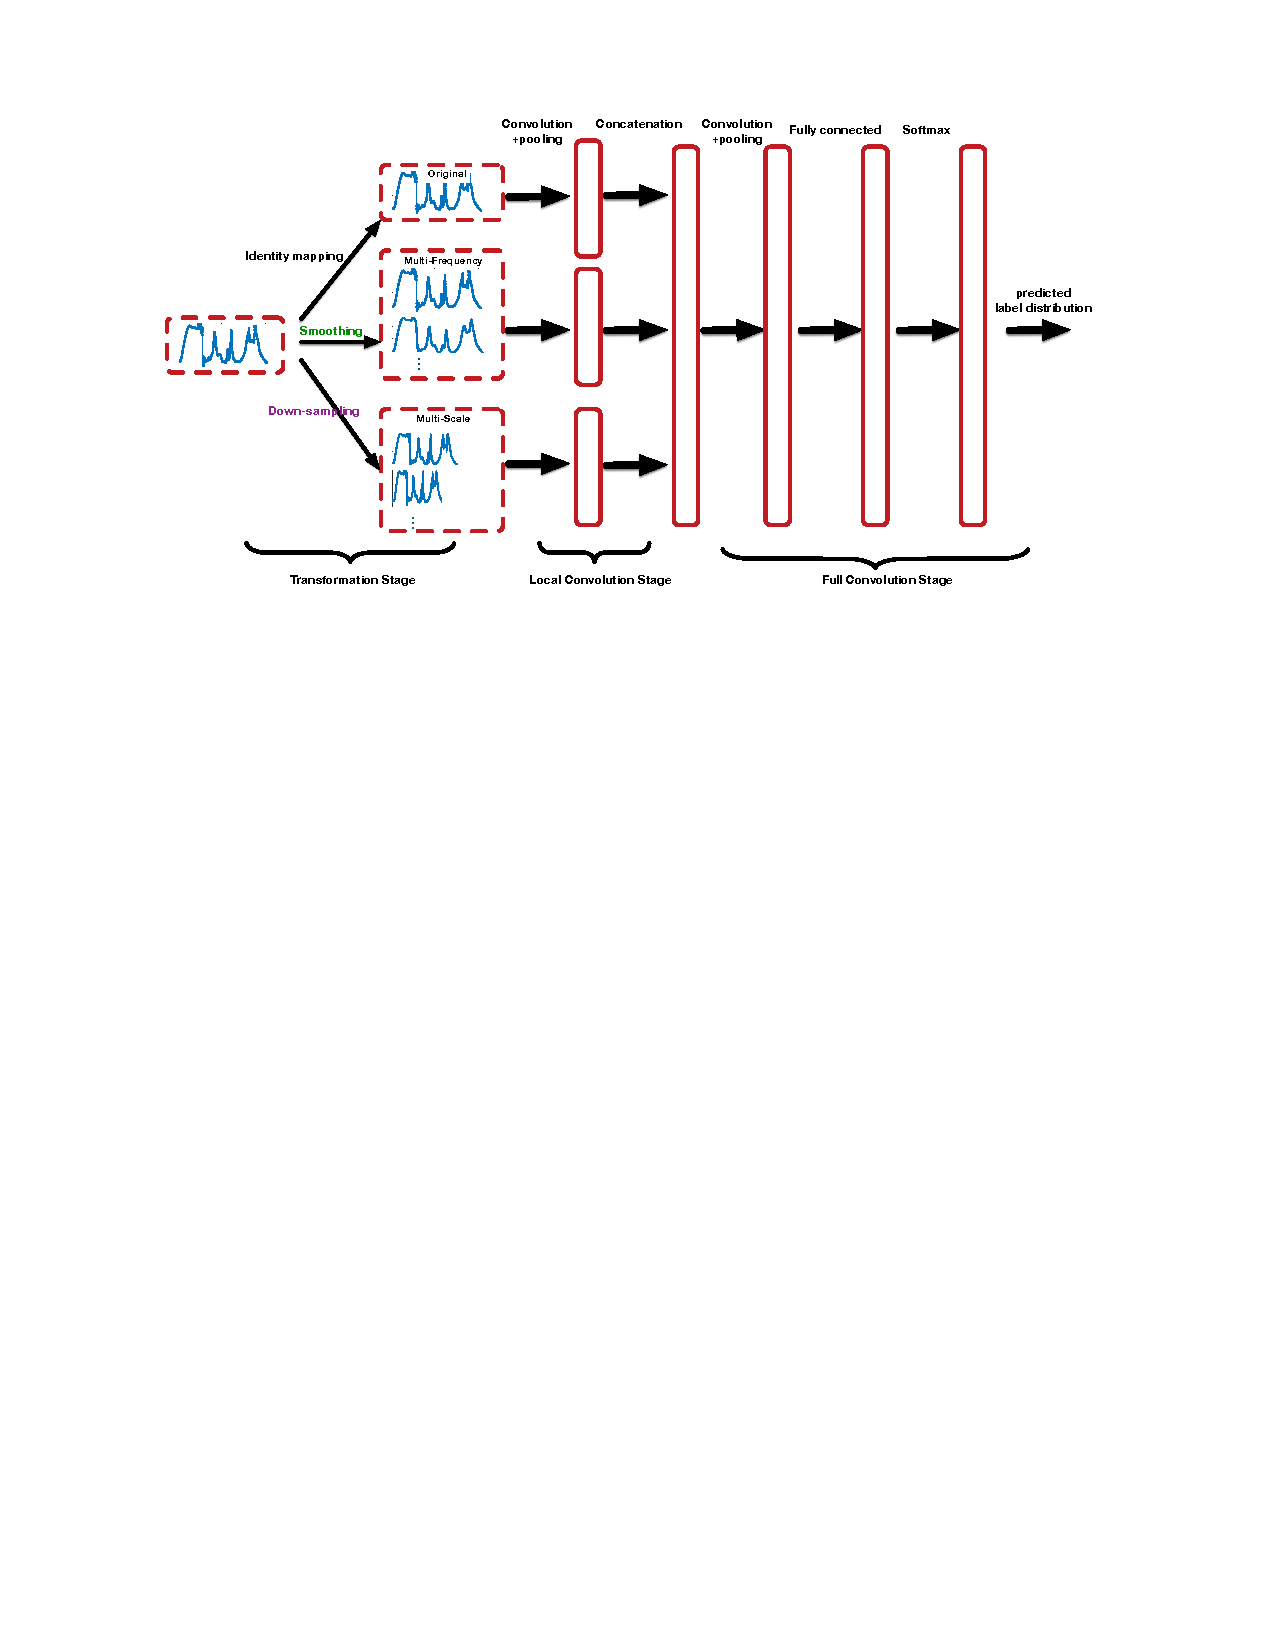
\includegraphics[width=.95\textwidth]{figure/mcnn}
	\end{center}
\end{frame}

\subsection{Time Le-Net}

\begin{frame}{Time Le-Net\footfullcite{le2016data}}
\framesubtitle{Inspired by Le-Net\footfullcite{lecun1998gradient},like CNN: 2 Conv + FC + final softmax}
\begin{columns}
	\column{.47\textwidth}
	Compared to FCN:\\
	GAP $\to$ {\color{red}FC}
	\begin{block}{Local max pooling}
		\begin{itemize}
			\item take max in a local pooling
			\item + invariance to small perturbations
			\item shorten a time series
		\end{itemize}
	\end{block}
	Still {\color{red}{\#parameters $\uparrow$}} \#invariance $\downarrow$
	\column{.5\textwidth}
	Data augmentation to prevent {\color{red}{overfitting}}
	{\color{gray}{especially on relatively small datasets}}
	\begin{block}{Window Slicing(WS)}
		= method used in MCNN
	\end{block}
	\begin{block}{Window Warping (WW)}
		For a time series with length $l$
		\begin{enumerate}
			\item dilate ($\times 2$) $\to 2l$
			\item squeeze ($\times \frac{1}{2}$) $\to \frac{1}{2}l$
 		\end{enumerate}
	\end{block}
\end{columns}
\end{frame}

\begin{frame}{Window Warping (WW)}
	\framesubtitle{Then feed all data (length=$l$,$2l$,$\frac{1}{2}l$) into network}
	\begin{center}
		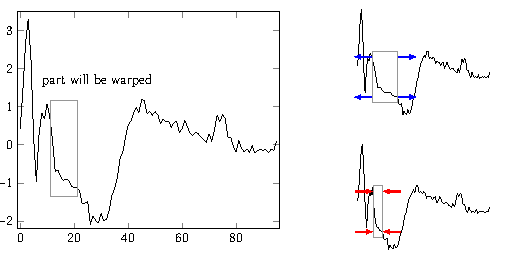
\includegraphics[width=.9\textwidth]{figure/ww}
	\end{center}
\end{frame}

\subsection{MCDCNN}

\begin{frame}{MCDCNN\footfullcite{zheng2014time}}
	\framesubtitle{Multi Channel Deep Convolutional Neural Network: \textbf{Independent} Conv specified for \textbf{MTS}}
	\begin{center}
		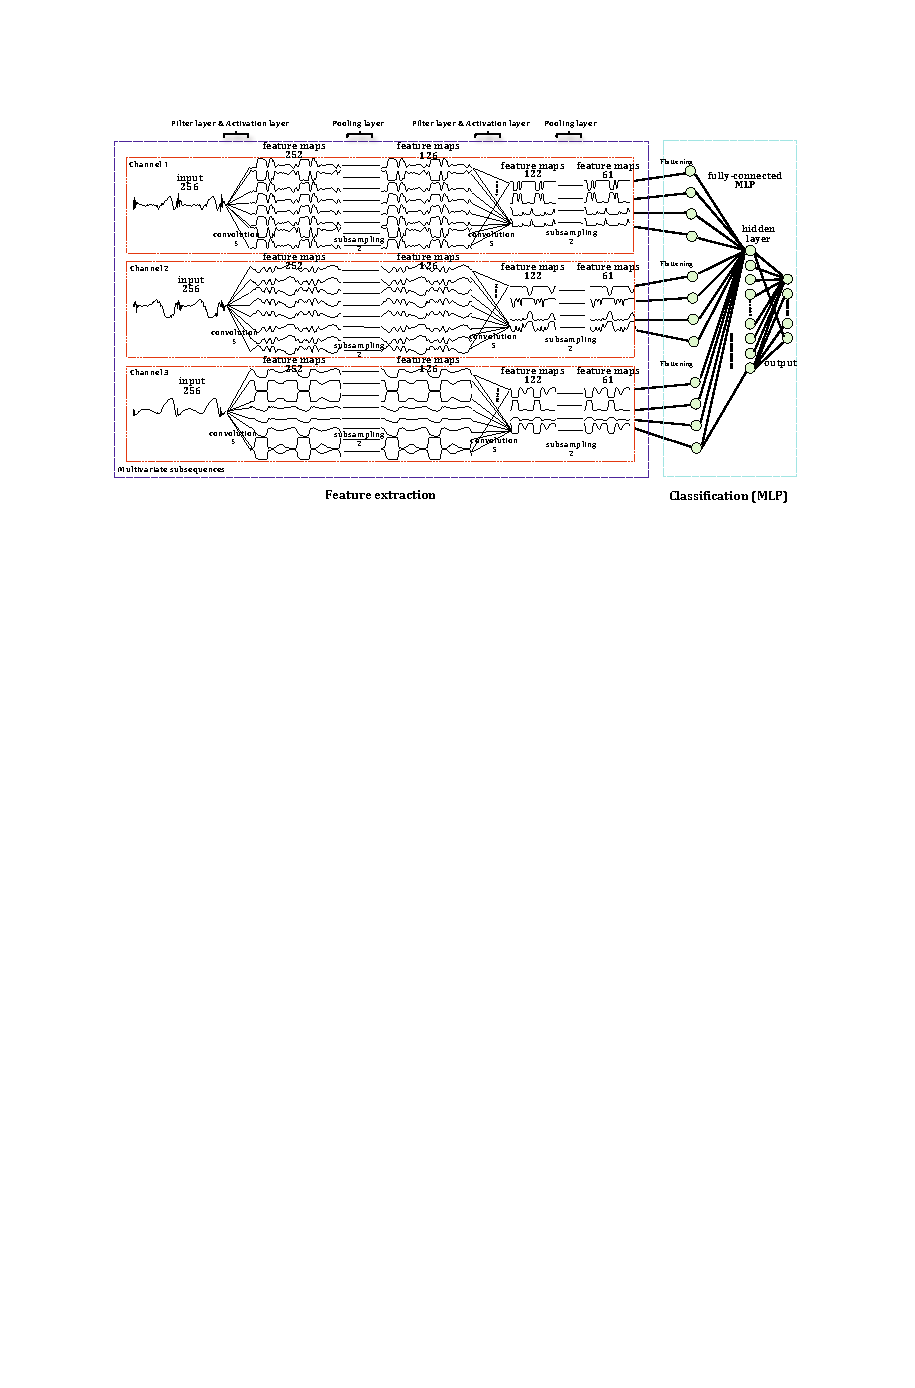
\includegraphics[width=.75\textwidth]{figure/mcdcnn}
	\end{center}
\end{frame}

\subsection{Time-CNN}

\begin{frame}{Time-CNN \footfullcite{zhao2017convolutional}}
	\framesubtitle{both for univariate and multivariate}
	Main differences compared to previous models:
	\begin{enumerate}
		\item loss function: categorical cross-entropy $\to$ MSE
		\item activate function of final layer: softmax $\to$ sigmoid
			$$\sum_{i=1}^{K}{p(\hat Y_{i})} \ne 1$$
		\item throughout CNN: local max pooling $\to$ local average pooling
	\end{enumerate}
	Compared to some models:
	\begin{itemize}
		\item apply 1 Conv for all dimensions (unlike MCDCNN)
		\item Conv directly fully connected to final layer (modify FCN: GAP $\to$ FC)
	\end{itemize}

\end{frame}

\subsection{TWIESN}

\begin{frame}{Echo State Network (ESN)\footfullcite{gallicchio2017deep}}
	\framesubtitle{Based on RNN}
	\begin{columns}
		\column{.6\textwidth}
		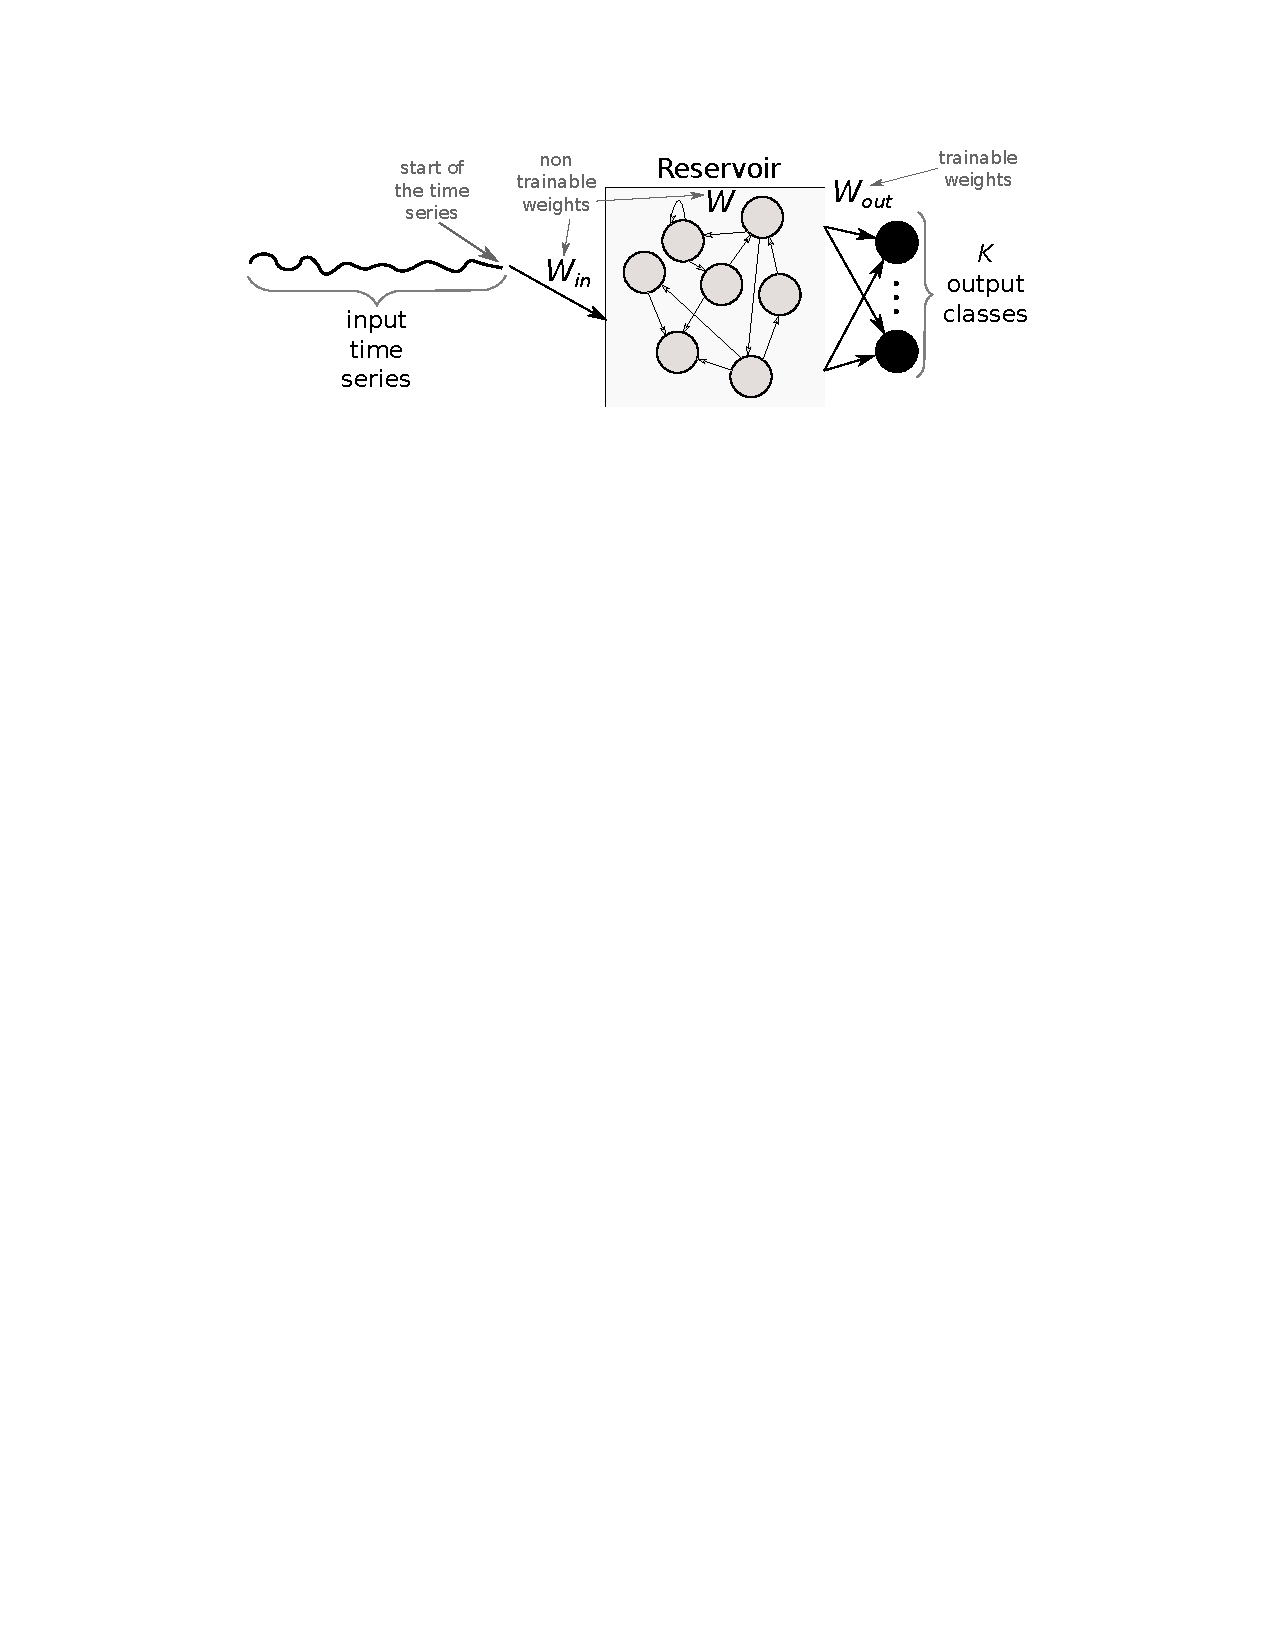
\includegraphics[width=\textwidth]{figure/esn}
		\column{.4\textwidth}
		Core part: reservoir
		\begin{itemize}
			\item sparsely connected random RNN
			\item each neuron create its own nonlinear activation of the incoming signal
		\end{itemize}
	\end{columns}
			Internal state at time $t$ : $I(t) \in R^{N_r}$, $N_r = $ \#neurons inside reservoir
			$$I(t) = \sigma (W_{\text{in}} X(t) + W I(t-1)) | \forall t \in [1,T]$$
			Finally
			$${\hat Y} (t) = W_{\text{out}} I(t)$$
\end{frame}

\begin{frame}{TWIESN\footfullcite{tanisaro2016time}}
	\framesubtitle{Time Warping Invariant Echo State Network}
	ESN orginally proposed for time series forecasting
	$\to$ predicts a probability distribution

	Training
	\begin{enumerate}
		\item reservoir space ($\forall t$): $X(t) \to$ \textbf{higher} dimensional space
		\item train a Ridge classifier to predict the class of each $X(t)$
	\end{enumerate}
	Testing
	\begin{enumerate}
		\item $\forall X(t)$, trained Ridge classifier predicts a probability distribution
		\item for each class $k$, calculate a posteriori probability
		\item label $k$ with the largest average probability
		$$\arg\max_{k}{\frac{1}{T}} \sum_{t=1}^{T} {\hat Y_k (t)}$$
	\end{enumerate}
\end{frame}

\begin{frame}{Summary}
	\begin{center}
		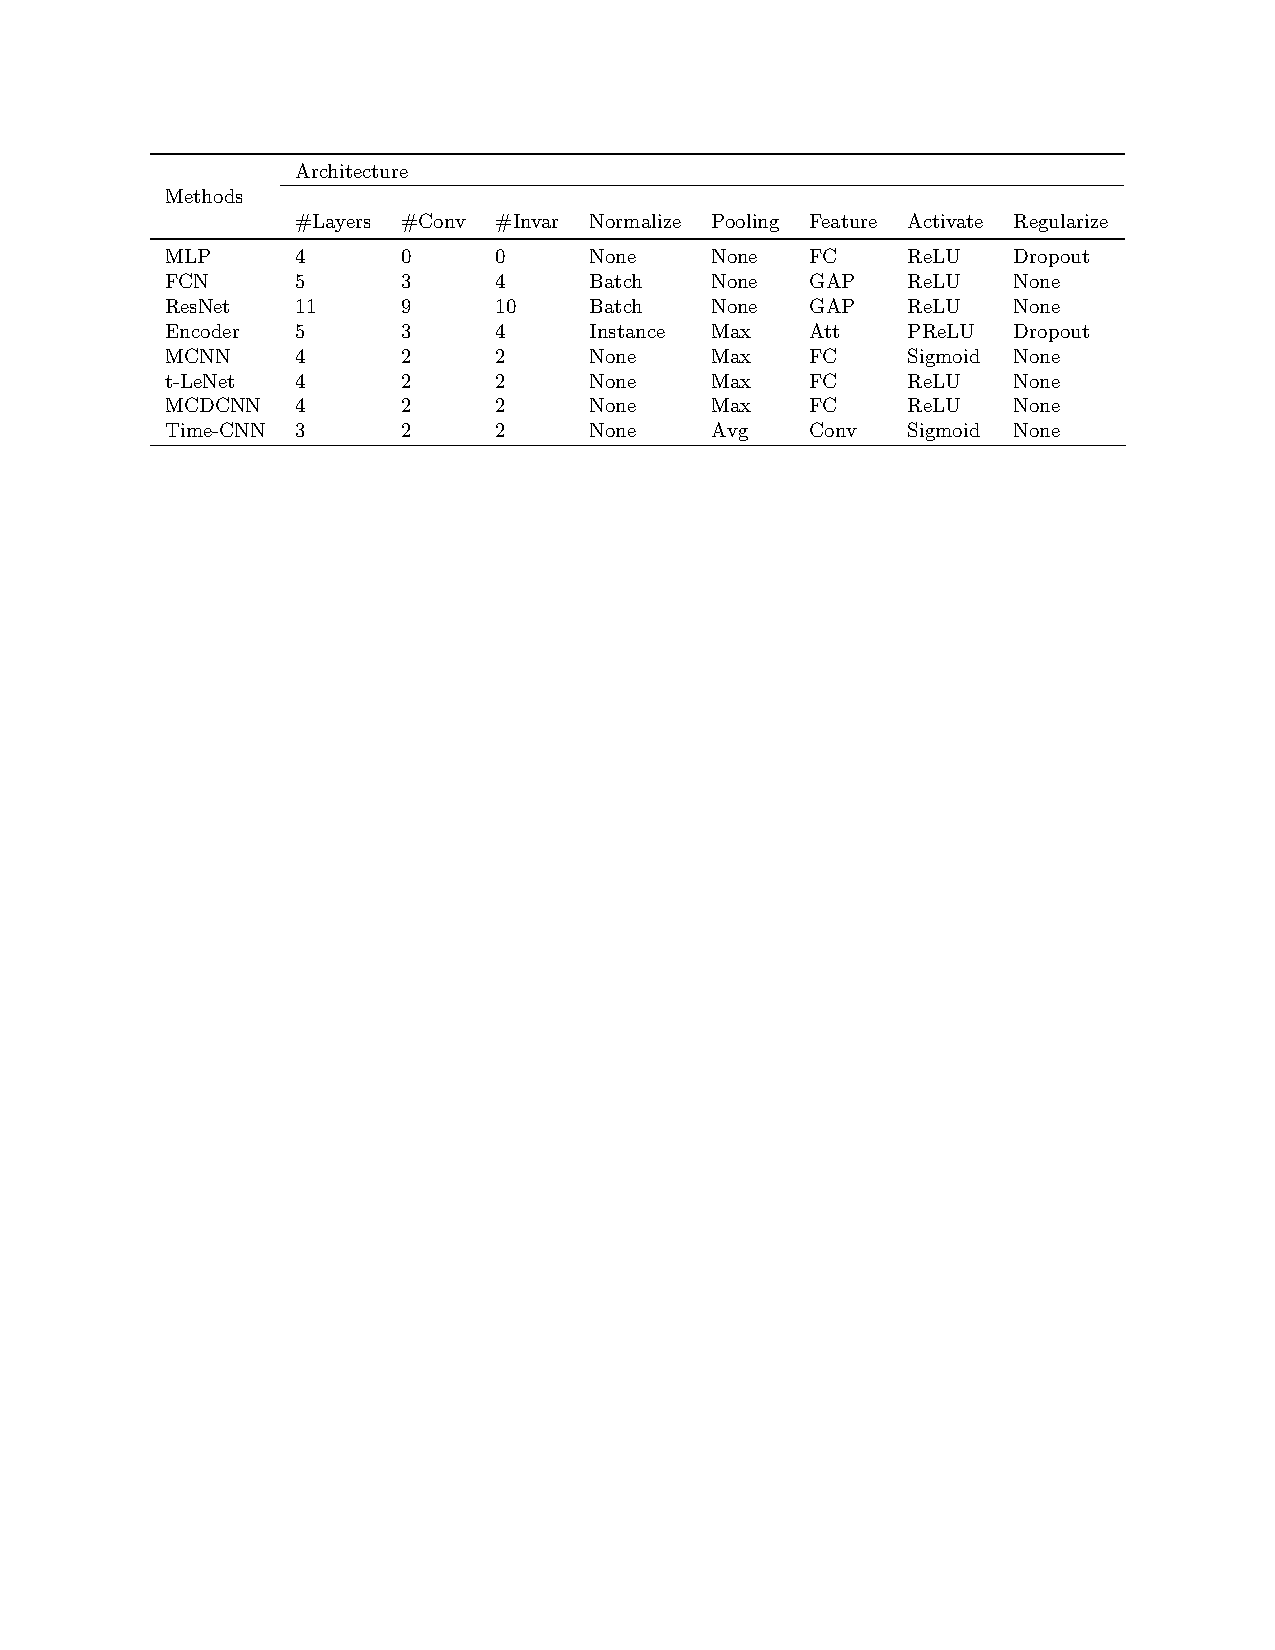
\includegraphics[width=1.05\textwidth]{figure/arch}
	\end{center}
\end{frame}

\section{结论}

\begin{frame}{Overall Performance}
	\framesubtitle{Critical Difference Diagram (dataset: UCR/UEA)}
	{\Large{\begin{description}[leftmargin=!]
		\item[univariate] 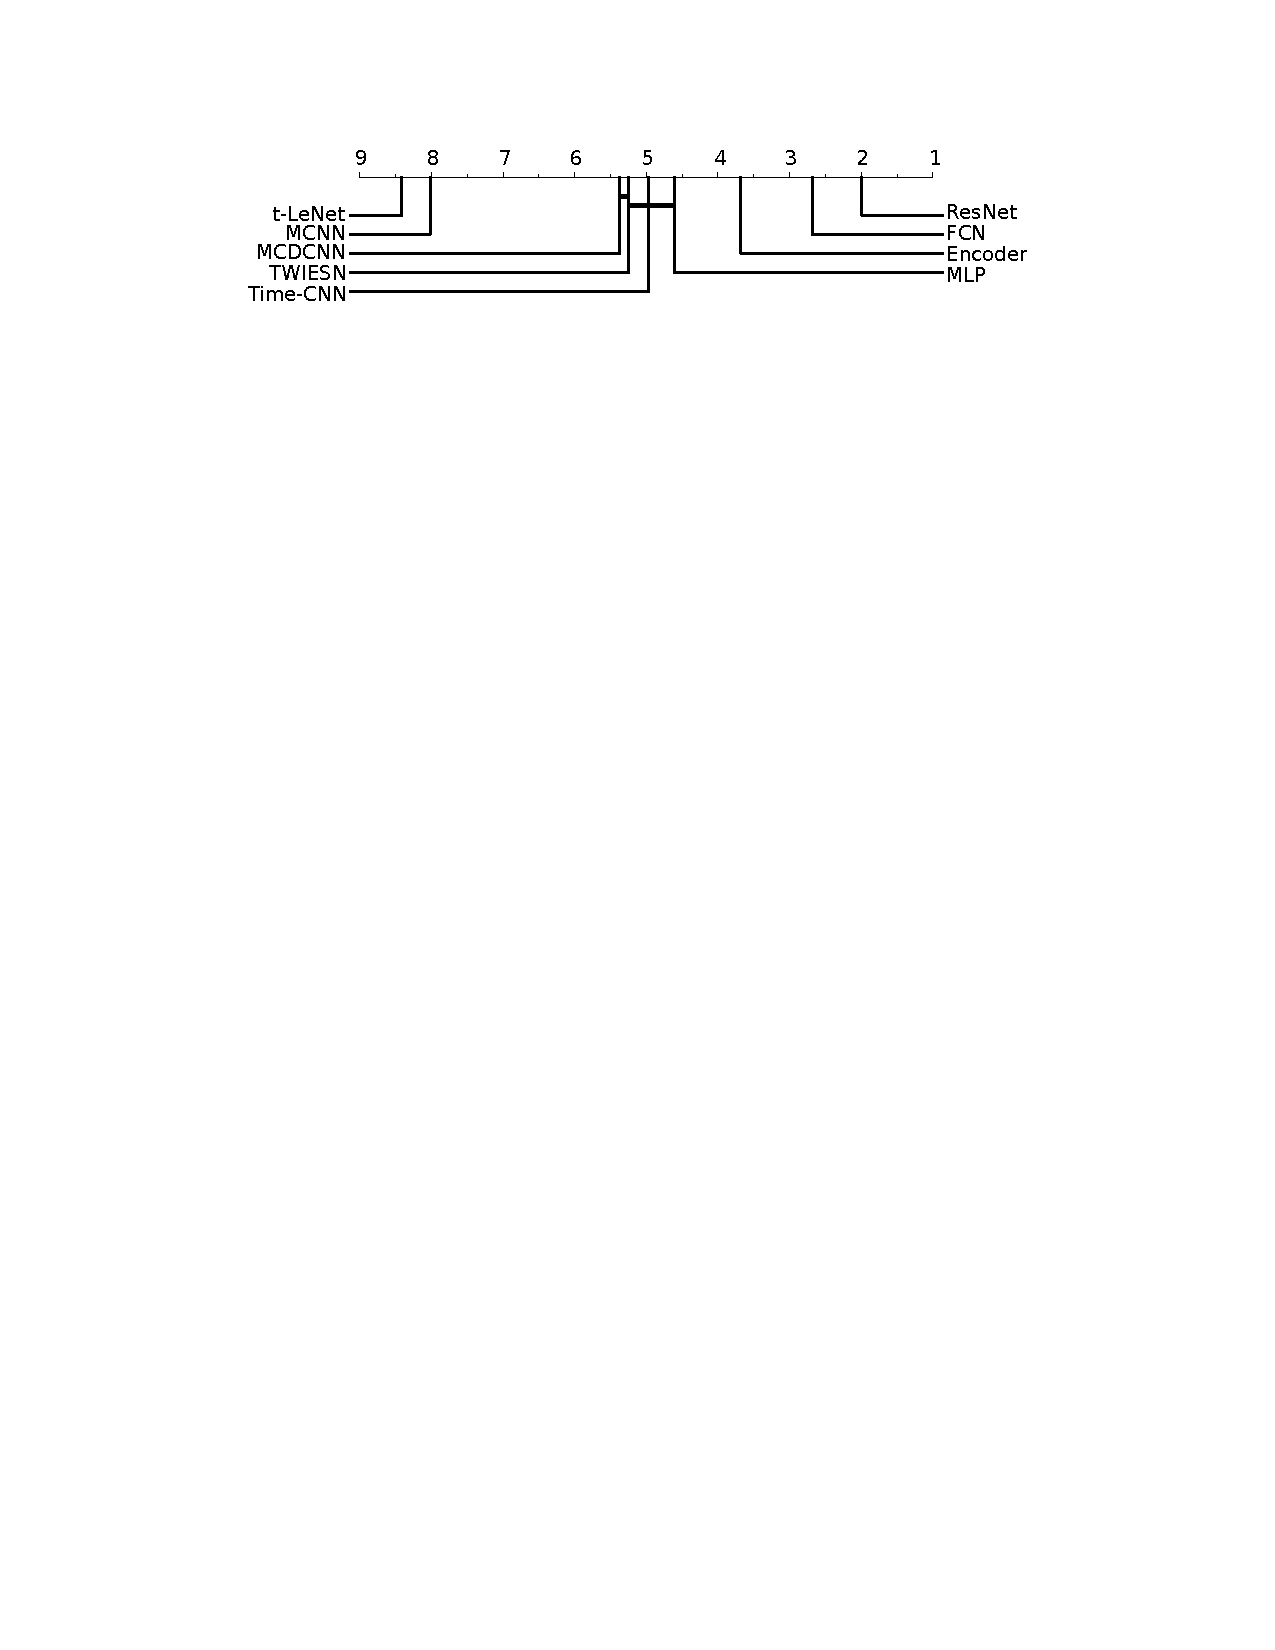
\includegraphics[width =.7\textwidth]{figure/uni_cd}
		\item[multivariate] 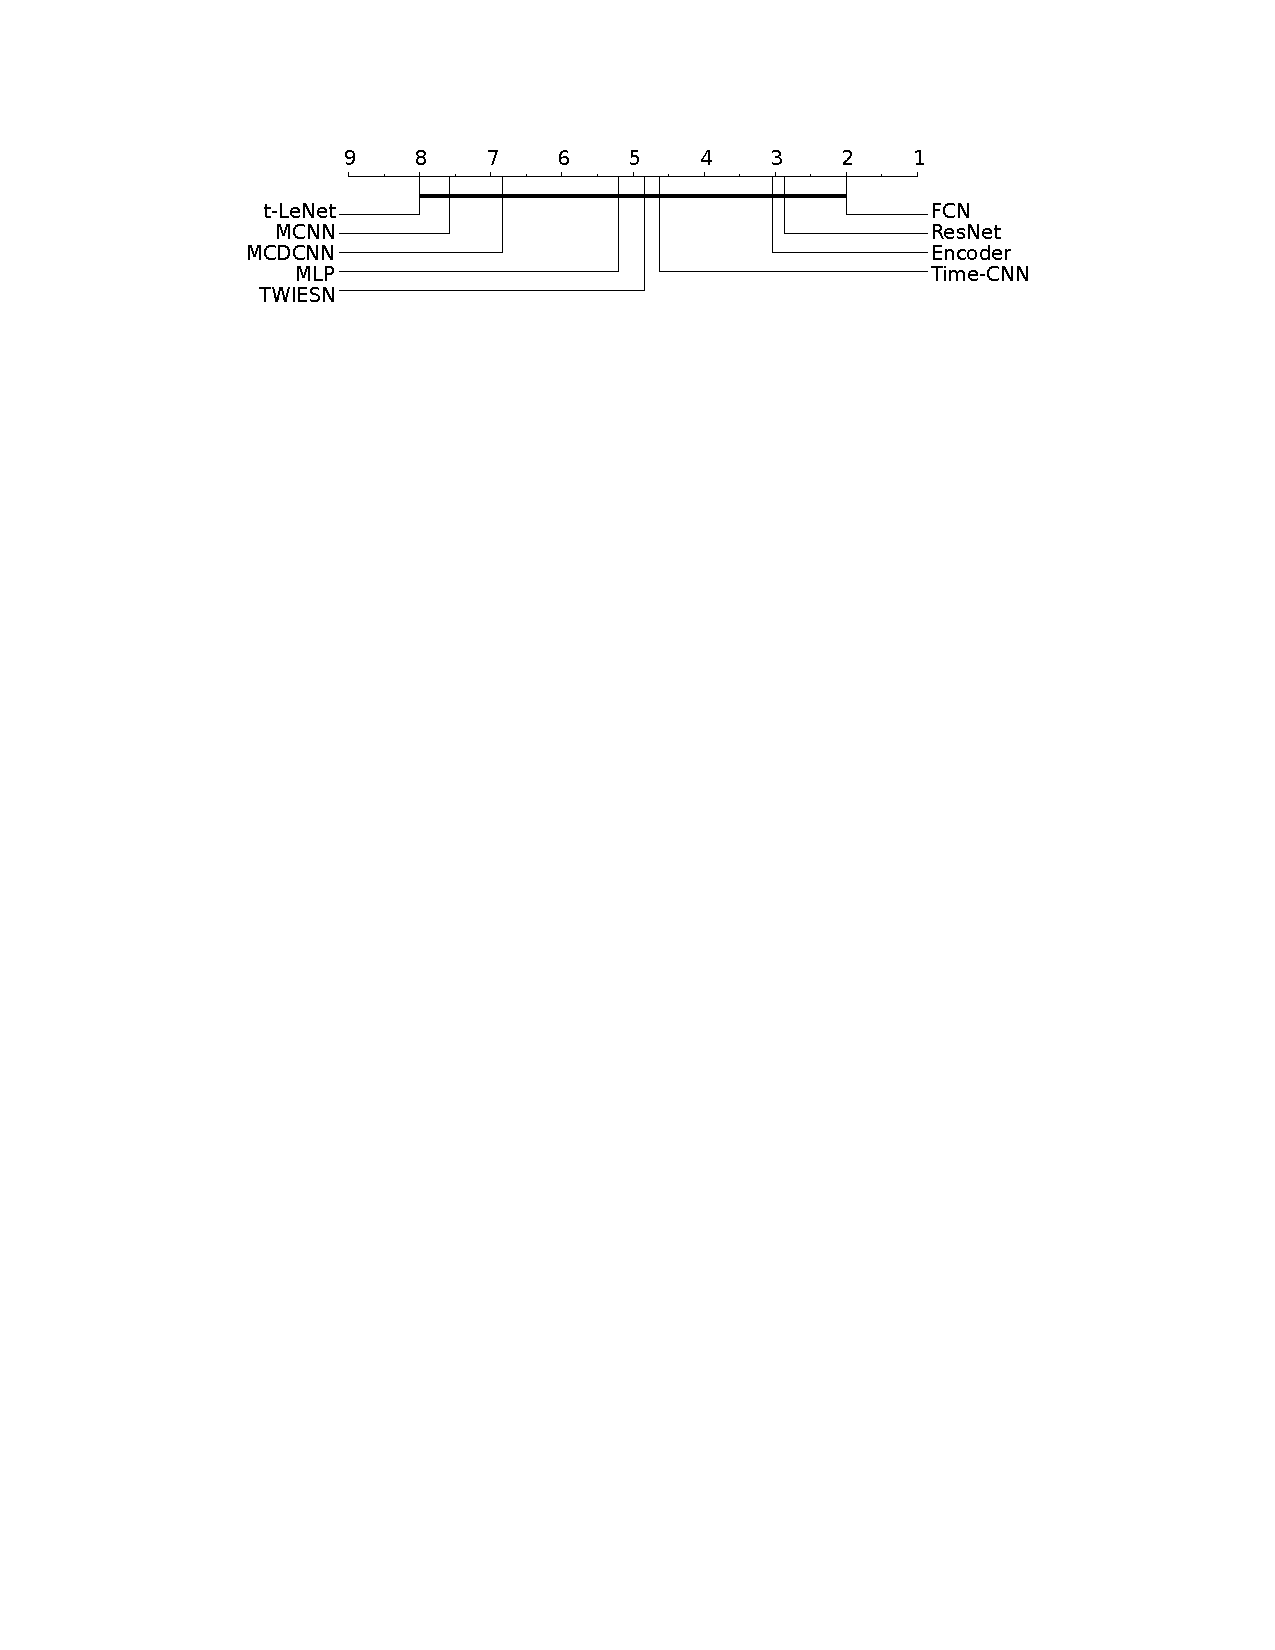
\includegraphics[width =.7\textwidth]{figure/multi_cd}
		\item[both] 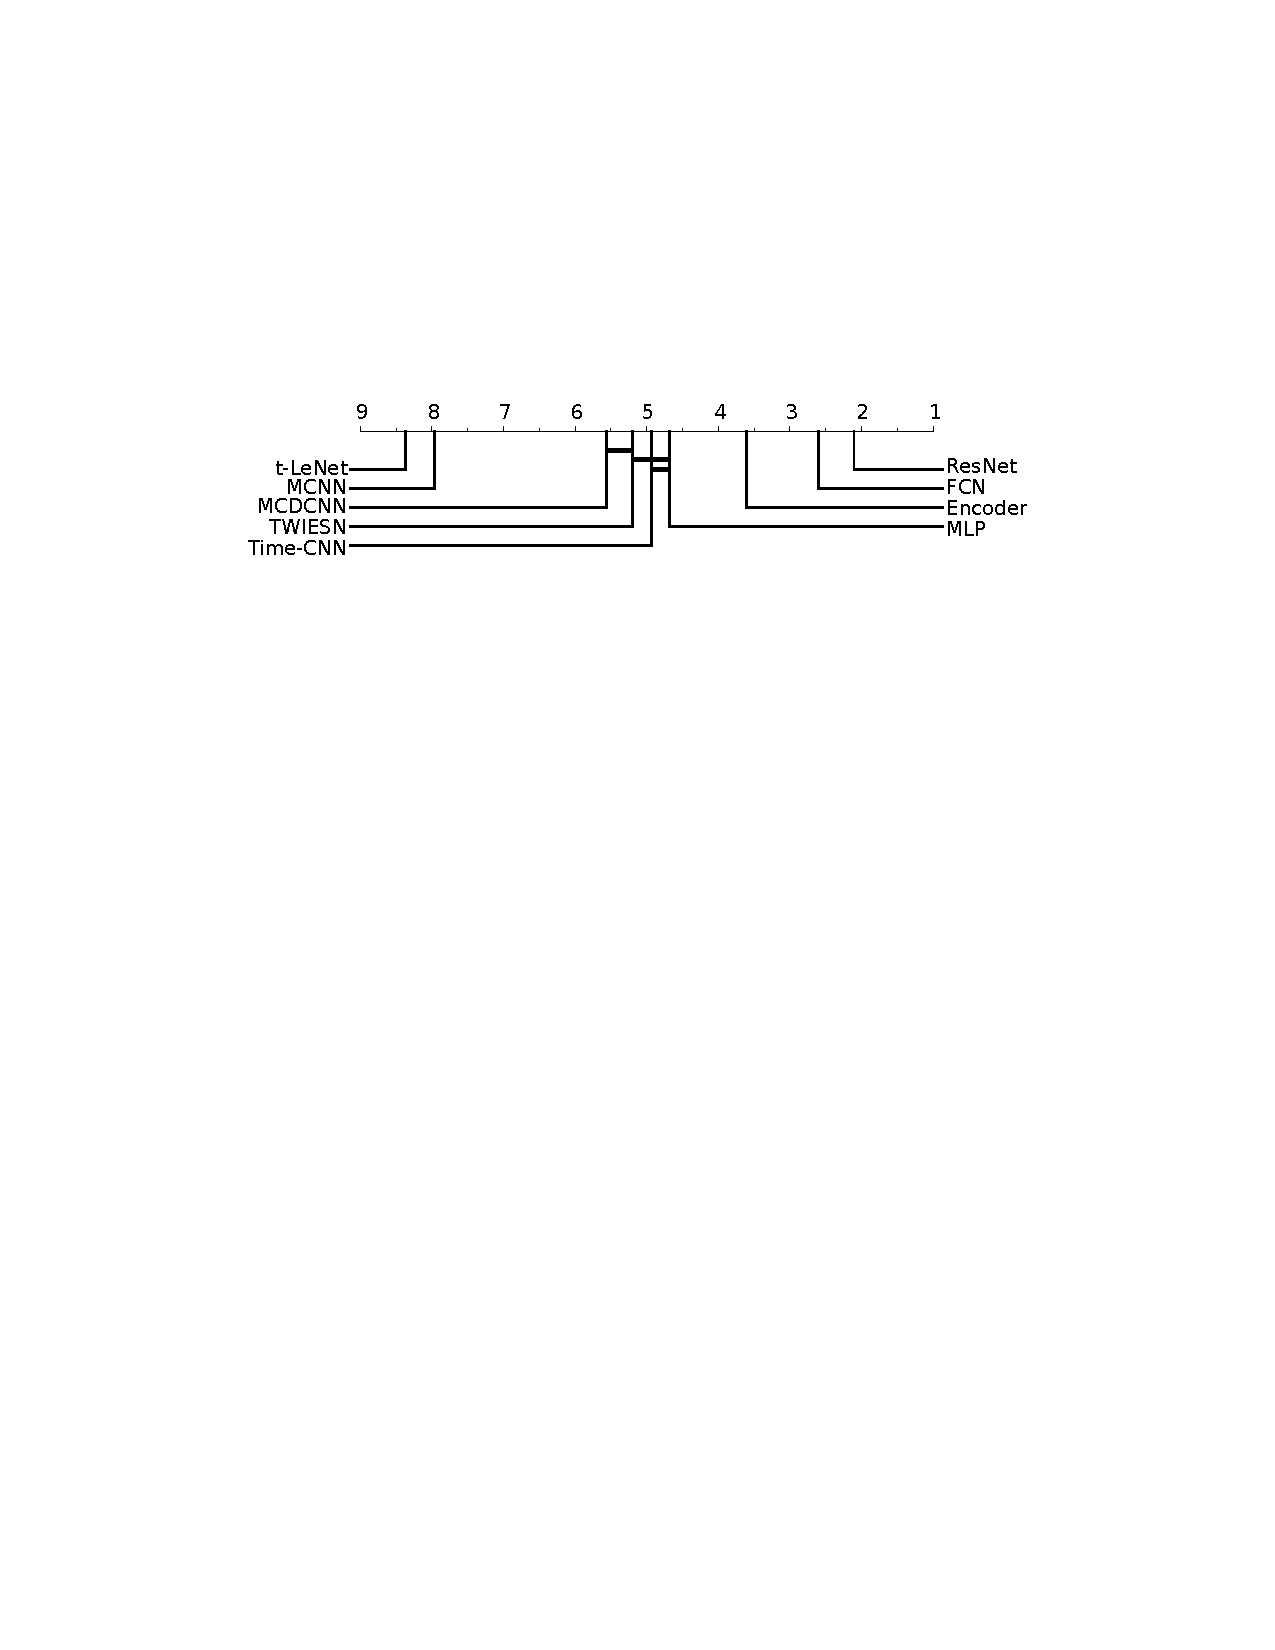
\includegraphics[width =.7\textwidth]{figure/both_cd}
	\end{description}}}
\end{frame}

\begin{frame}{For Different Datasets}
	\begin{center}
		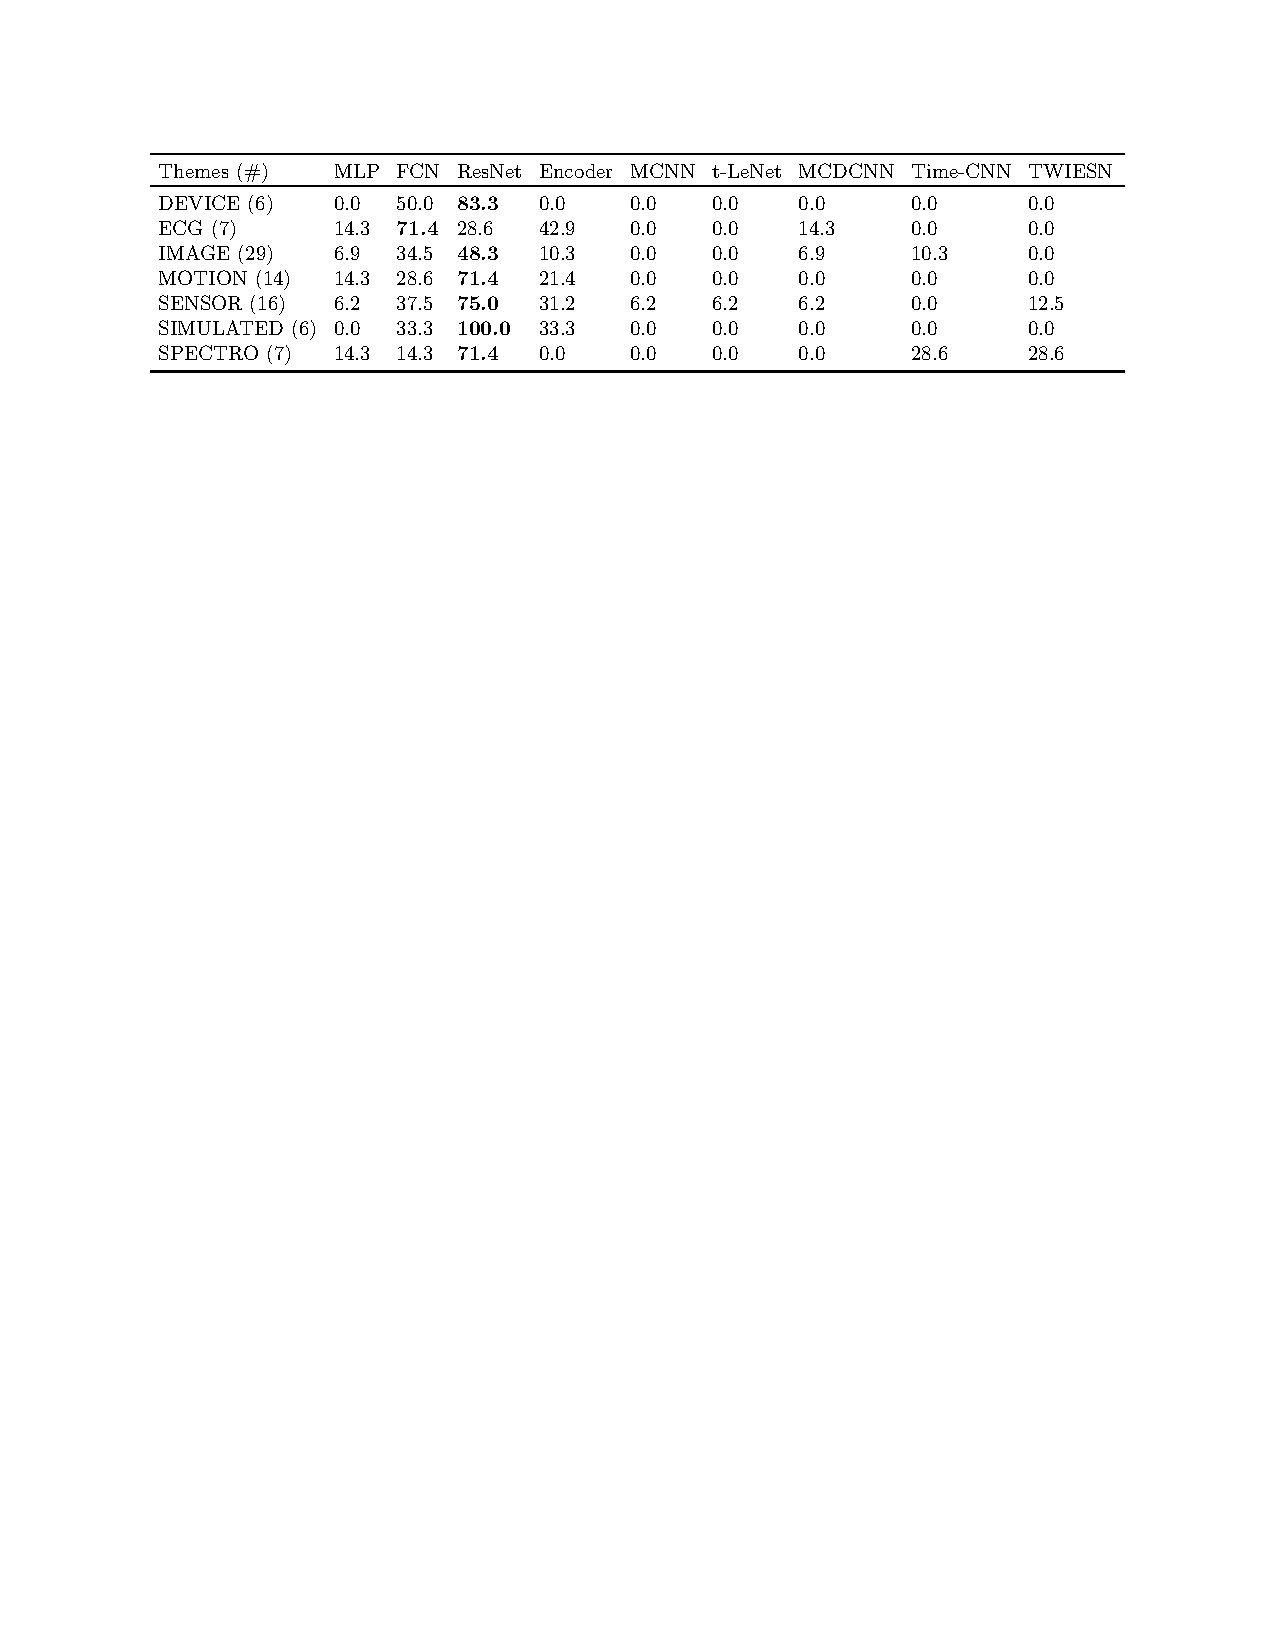
\includegraphics[width=\textwidth]{figure/theme}
	\end{center}
\end{frame}

\begin{frame}{}
	\begin{center}
		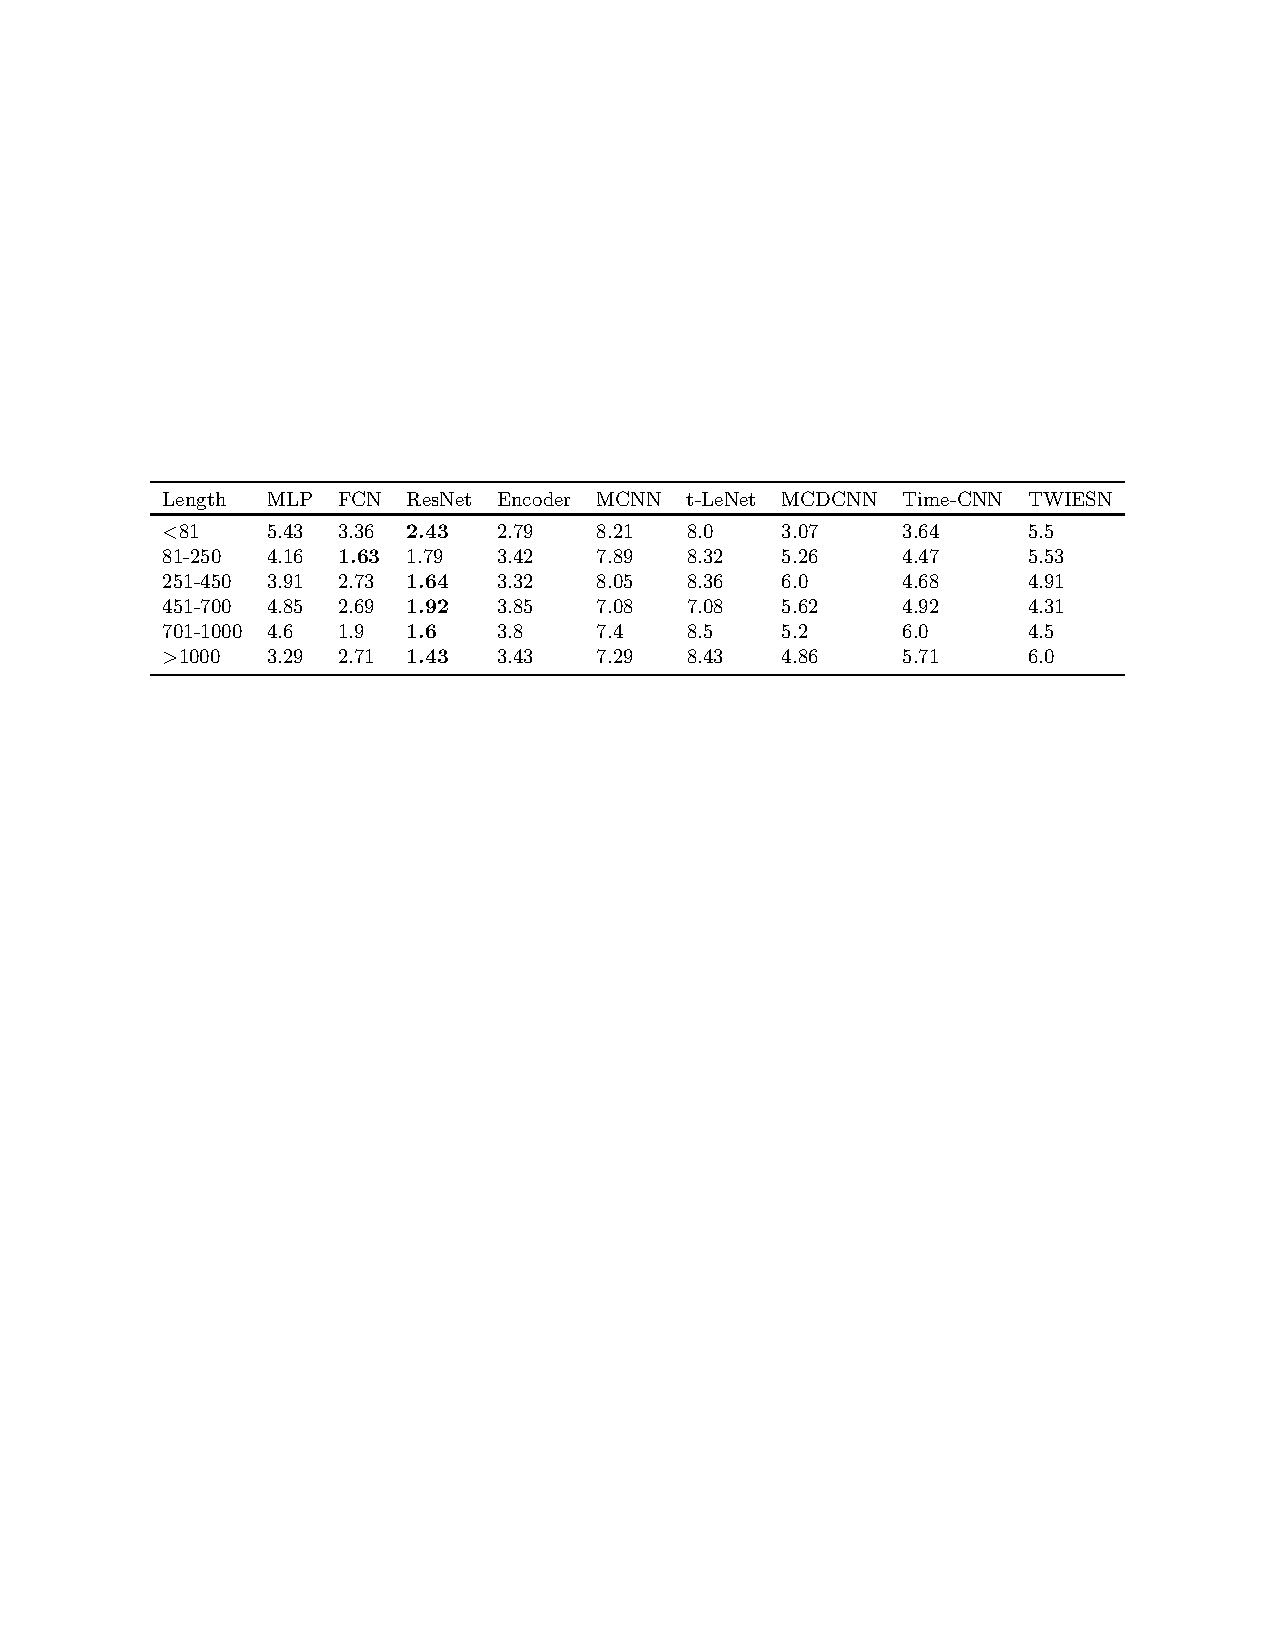
\includegraphics[width=\textwidth]{figure/length}
		\\
		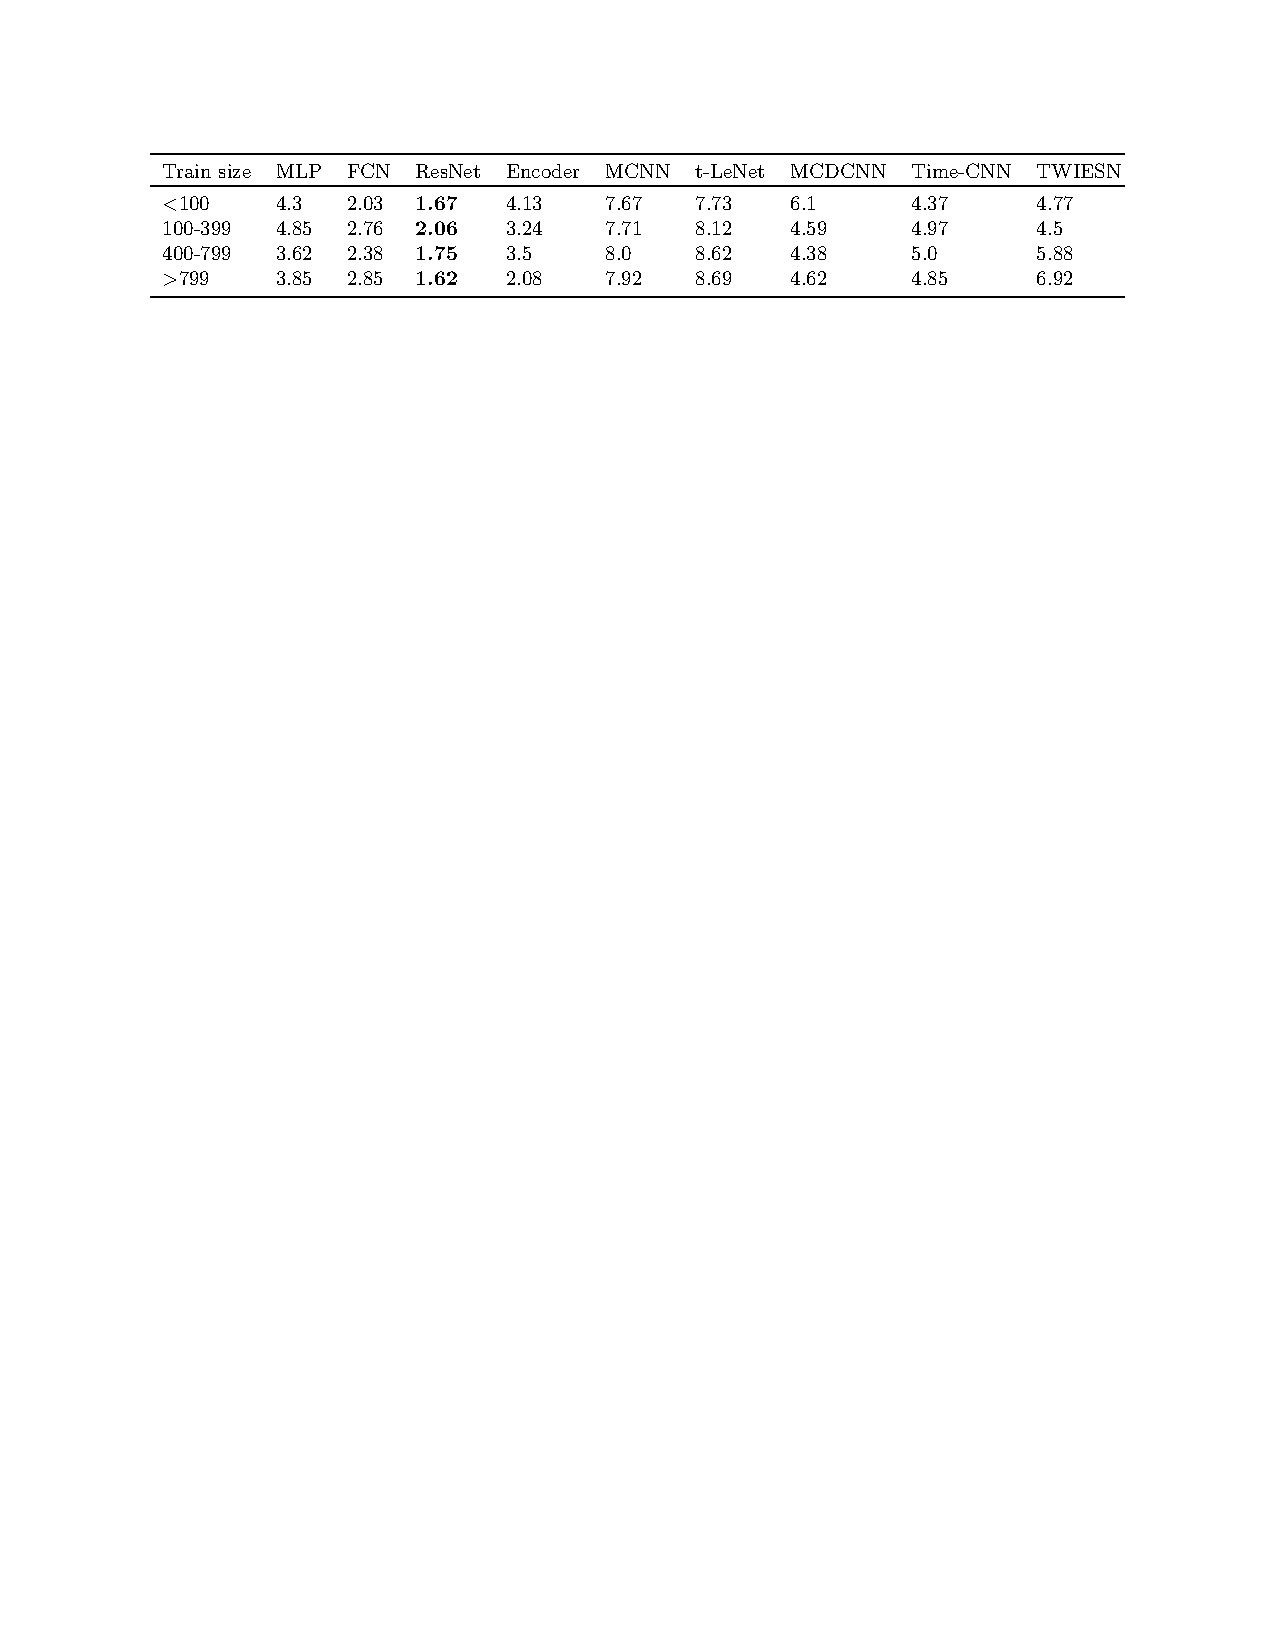
\includegraphics[width=\textwidth]{figure/train_size}
	\end{center}
\end{frame}

\subsection{Visualization Reasoning}

\begin{frame}{Class Activation Map (CAM) \footfullcite{zhou2016learning}}
	\framesubtitle{GAP layer + softmax}
	univariate time series $A_{m}(t)$ produced by $m$-th filter in Last Conv, input to neuron of class $c$
	$$\begin{aligned}
			z_c & = \sum_{m}{{w_m}^c \sum_{t}{A_m(t)}} \\
			    & =  \sum_{m}{\sum_{t} {{w_m}^c A_m(t)}}
		\end{aligned}$$
	Therefore, $CAM_c$ that explains the classification as label $c$
	$$CAM_c (t)= \sum_{m}{{w_m}^c A_m(t)}$$
	constructed a new time series for further observation and explaination.
\end{frame}

\begin{frame}{Find discriminative Region}
	\framesubtitle{Example: FCN/ResNet on GunPoint dataset (achieve 100\% accurancy)}
	\begin{center}
		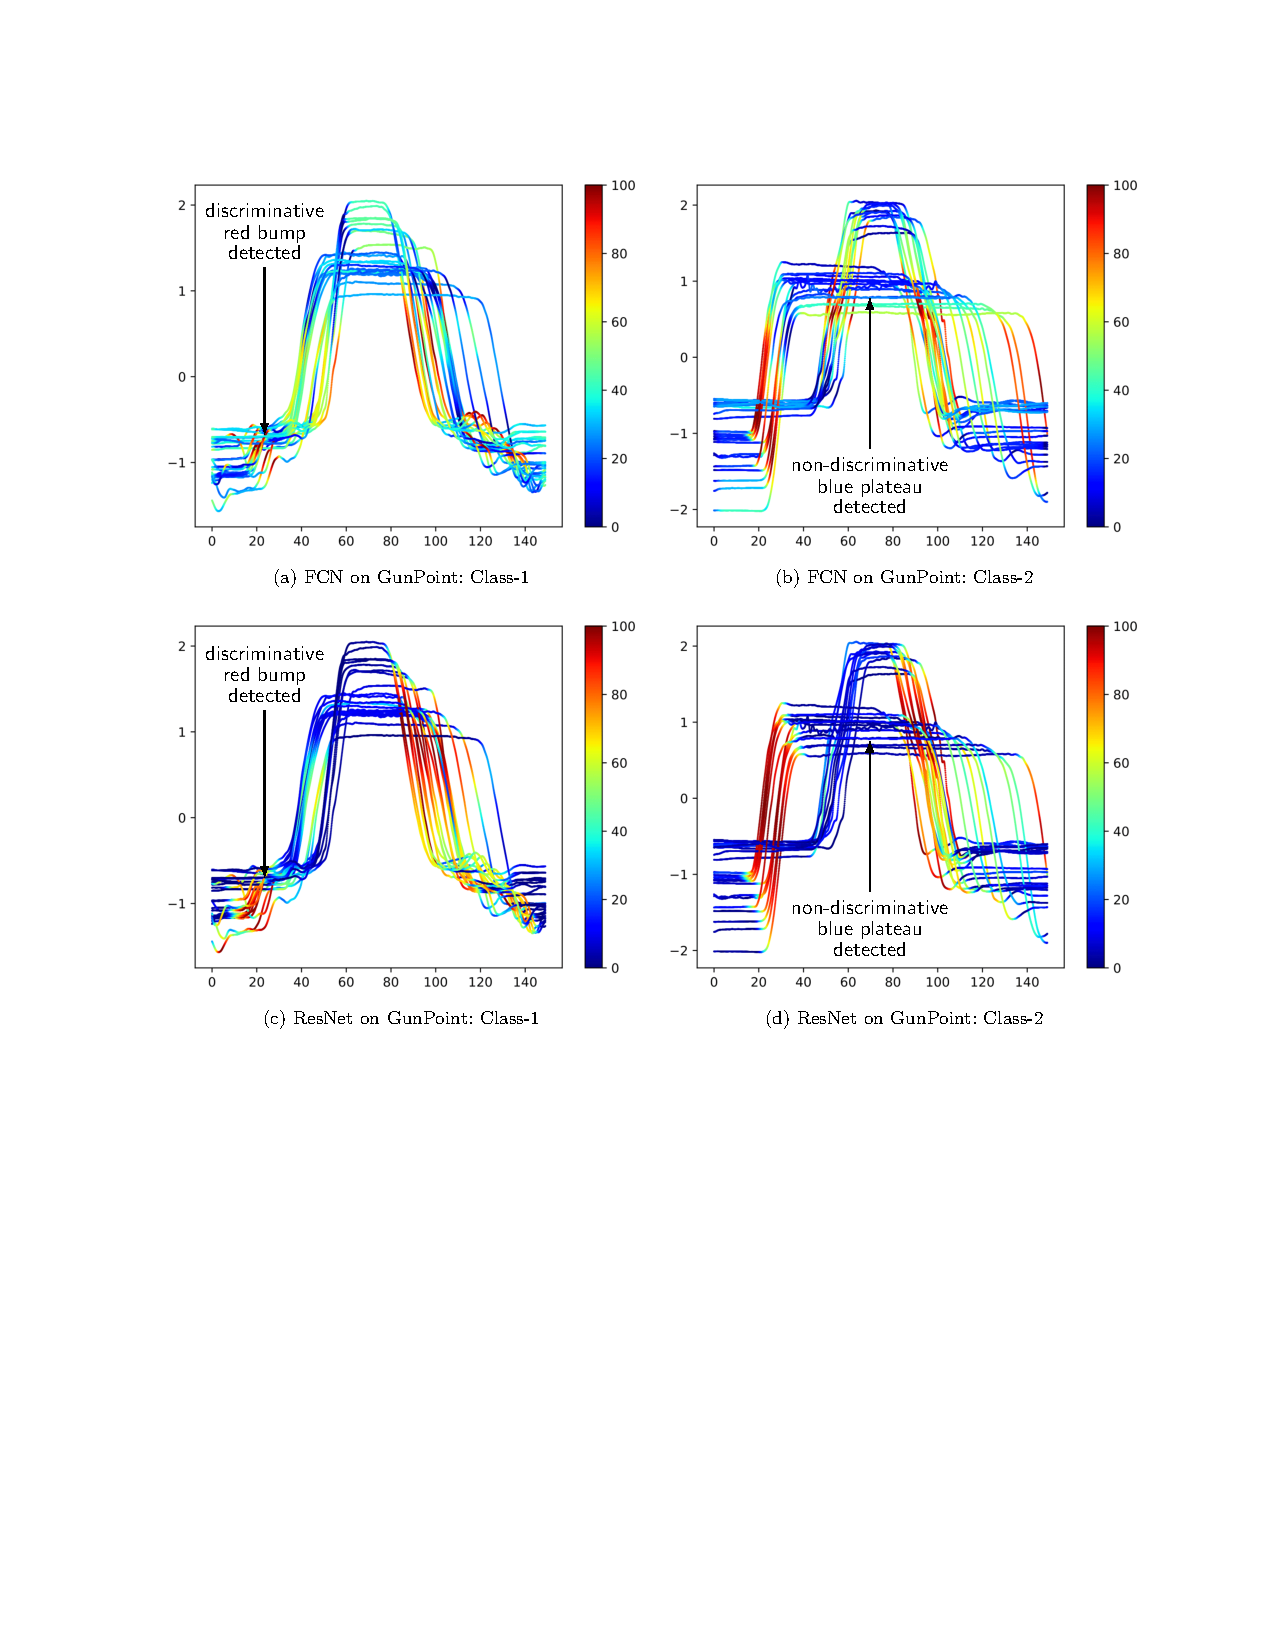
\includegraphics[width=.6\textwidth]{figure/cam_example}
	\end{center}
\end{frame}

\section{TSC社区生态}

\begin{frame}{Libraries/Implements/Community}
  \framesubtitle{sktime\footfullcite{sktime} \& its extensions}
  \href{https://github.com/alan-turing-institute/sktime}{\Large{Sktime}}
  \begin{itemize}
    \item based on classic models (shallow)
    \item \texttt{scikit-learn} interface compatible
  \end{itemize}
  \href{https://github.com/sktime/sktime-dl}{\Large{Sktime-dl}}
  \begin{itemize}
    \item use \texttt{Keras} to implement all 9 deep models above
    \color{red}{\item 暂时\textbf{不能}直接安装(MacOS)}
  \end{itemize}
  \href{http://www.timeseriesclassification.com/}{\Large{UEA \& UCR Time Series Classification Repository}}
  \begin{itemize}
    \item 128 TSC datasets + 30 MTS datasets
    \item Collect a bunch of \textbf{classic} algorithms
  \end{itemize}
\end{frame}

\begin{frame}{}
  \begin{center}
  {\Huge{Thanks}} \\
  All codes, slides and papers available\\
  \faGithub \href{https://github.com/li-xin-yi/deep_time_series_share_slide}{li-xin-yi/deep\_time\_series\_share\_slide}
\end{center}
\end{frame}

\end{document}
